\chapter{Fact-Checking}

\section{Task Description}

We see fact-checking as a crucial part of journalism, being the means of covering important events truthfully. 
The goal is to compare the reported fact or claim to the current state of the world or its assumed truthful approximation, in our case, the corpus of \CTK{} news articles (\CTK{} infobank) and the Czech Wikipedia.
We refer to this textual world-state representation as the knowledge base.
From the comparison, we can ``check'' the claim's truthfulness, proclaiming it true, false, or unverifiable. 
Thus, we can think of the task of fact-checking as a classification problem with labels True, False, and Not Enough Info (NEI). 
The claims are usually one or a few sentences long strings stating some fact or facts. 
There are platforms, such as Demagog.cz, which also use a category labeled ``misleading'', reserved for statements that are technically true but imply additional, false meaning.
For now, our models do not use this category, although it may be used in further research.

\begin{figure}[h!]
    \centering
    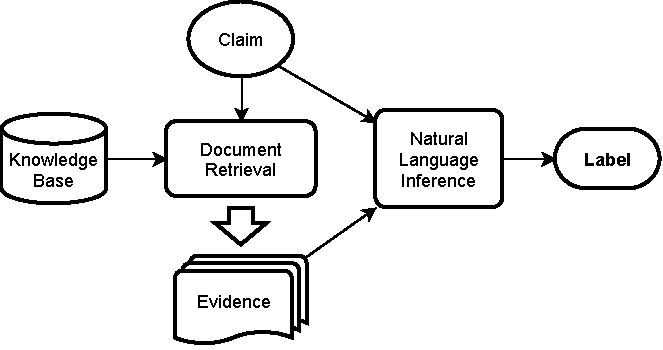
\includegraphics{fc_pipeline_label.pdf}
    \caption[Fact-Checking Pipeline]{Fact-checking pipeline diagram.}
    \label{fig:pipeline}
\end{figure}

To label a claim true or false, we also need to provide evidence validating or refuting the claim.
For our uses, the evidence is one or multiple news articles in \CTK{} infobank, which we consider an adequate approximation to the actual world state.
The infobank naturally provides a somewhat distorted image of reality since the journalists already assume some world knowledge, and the article form may further compress the original information.
Therefore, approaches based on language comprehension face the challenge of inferring real-world knowledge from somewhat distorted data. 

The above-described approach can be formulated as a sequence of subtasks (pipeline) depicted in Figure \ref{fig:pipeline}. The first step is to retrieve a collection of relevant documents from the knowledge base. This step is called document retrieval. Then, the Natural Language Inference task is performed, classifying the claim based on the selected documents.

\section{Related Work}

There exist several traditional fact-checking projects such as Demagog\footnote{\url{https://demagog.cz}}, PolitiFact\footnote{\url{https://www.politifact.com/}}, Factcheck.org\footnote{\url{https://www.factcheck.org/}}, and Washington Post Fact Checker\footnote{\url{https://www.washingtonpost.com/news/fact-checker/}}, with focus on fact-checking politicians' claims as well as general viral news. 

\begin{figure}[h!]
    \fbox{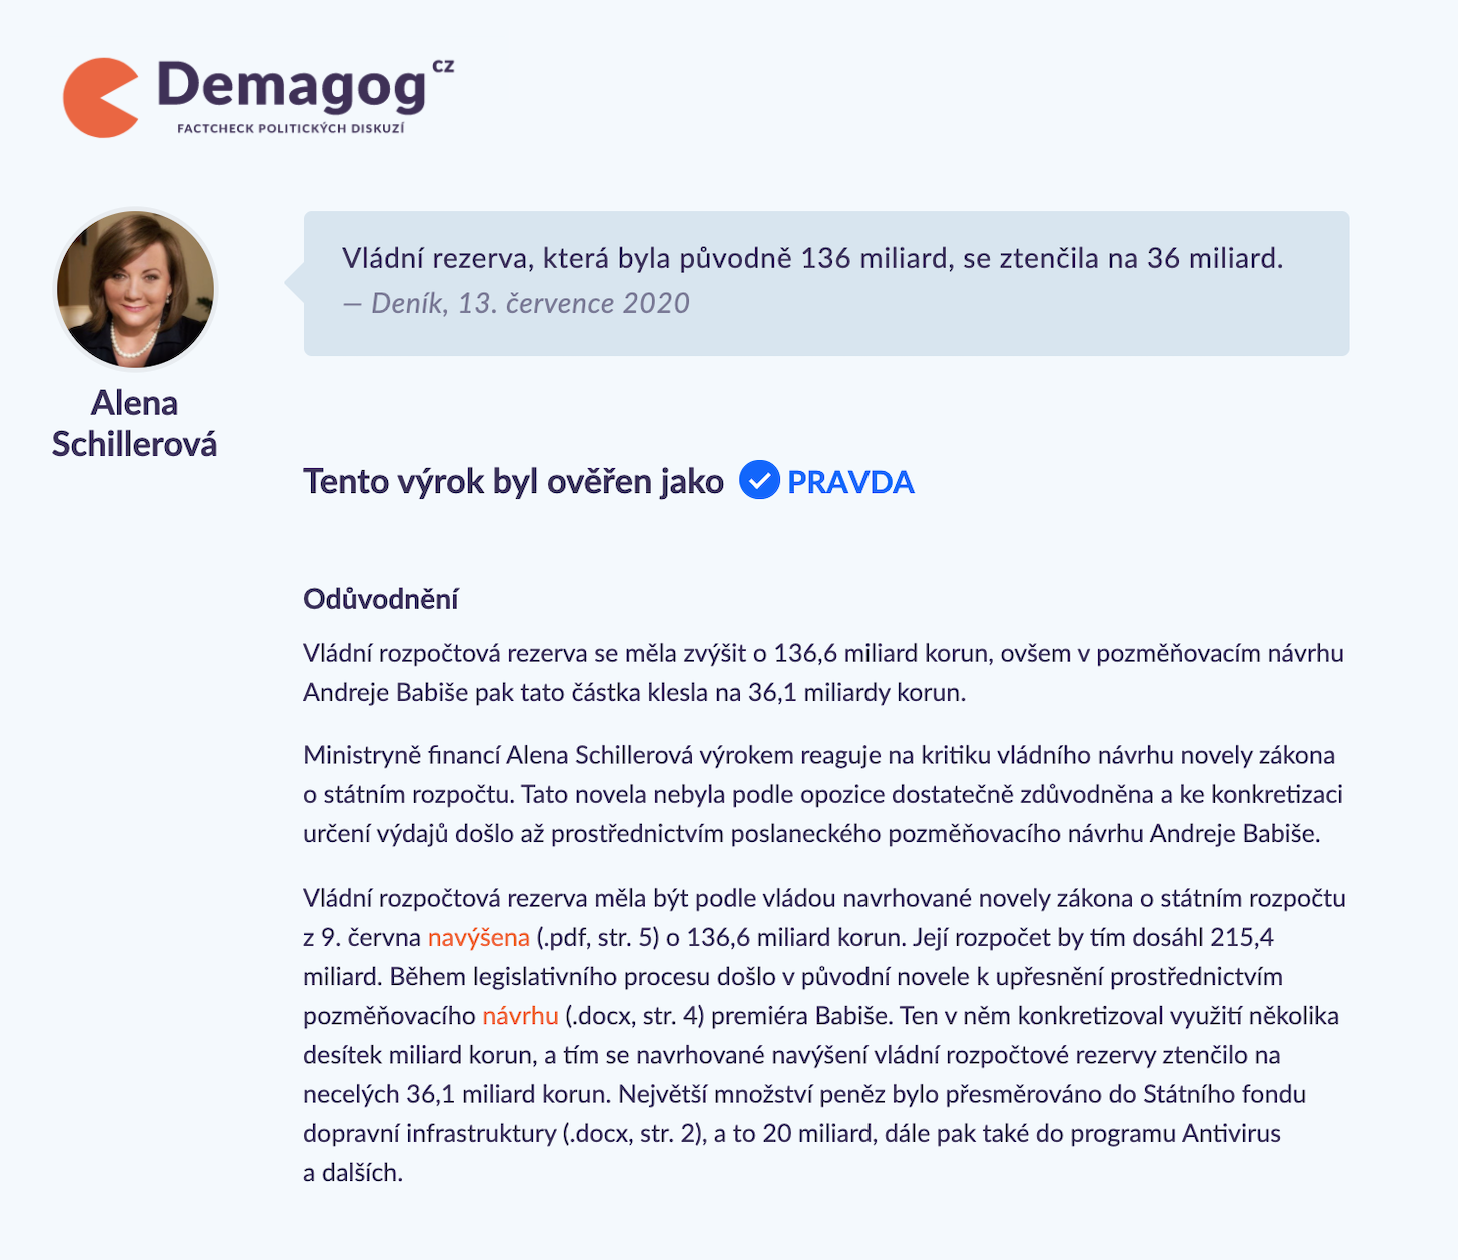
\includegraphics[width=142mm]{demagog.png}}
    \caption[Czech Demagog Entry Example]{Example claim, verdict, and its justification from the Czech Demagog project. Available at a permanent address \url{https://demagog.cz/vyrok/19500}.}
\end{figure}

Regarding automatic fact-checking, as of the time of writing, we are not aware of any other Czech fact-checking datasets other than \citep{czech-fact}.

Regarding the English language, \citet{fever} created the Fact Extraction and Verification (FEVER) dataset; the first large-scale dataset focused on open-domain fact-checking.
The pipeline (Figure \ref{fig:pipeline}) also appears in \citep{fever}, with the addition of the Sentence Selection step, where sentences forming the evidence are extracted after the document retrieval step.

The authors of the FEVER dataset also announced a shared task \citep{fever-2018-shared-task} in which ``The task challenged participants to classify whether human-written factoid claims could be \texttt{SUPPORTED} or \texttt{REFUTED} using evidence retrieved from Wikipedia.'' The results presented in \citep{fever-2018-shared-task} confirmed the pipeline approach, as the best performing submissions adhered to the design. T he authors continue organizing shared tasks with various modifications, such as \citep{fever-2019-shared-task-adversial}, with claims designed to mislead the models, and the current task\footnote{\url{https://fever.ai/task.html}(accessed 26th July 2021)}, focusing on a combined structured (tables present in articles) and unstructured (articles' texts) knowledge base.

%The fact-checking task is similar to the question answering (QA) task in retrieving the evidence. 
% However, QA queries (claims) are often made of very relevant words and thus naturally contain cues for finding relevant documents.

%%%%%%%%%%%%%% DON'T USE THIS PSEUDO-DEEP LOLOTHING %%%%%%%%%%%%%%%%%%
% This creates a perceived weakness that some might criticize, that we still rely on some "outside truth", and cannot decide what is objectively true. 
% Since something can be true only in relation to some other facts (the real state of the world, available news sources, etc.) this criticism lacks substance, but still emphasizes the importance of correclty choosing the knowledge database. 
% In our project, the knowledge database is the \CTK{} infobank. 

